\documentclass
% [landscape]
{article}

\usepackage{ctex}
\usepackage{amsmath}
\usepackage{graphicx}
\usepackage{epstopdf}
\usepackage{tikz}
\usepackage{psfrag}
\usepackage{natbib}
\usepackage{hyperref}

\begin{document}

\renewcommand{\refname}{参考文献}
\renewcommand{\figurename}{图}
\renewcommand{\abstractname}{摘要}
\def\due{2023 年 3 月 31 日周五 08:40}

\title{函数/数据/图形---规范及第1次作业 \footnote{2023 春季《磁流体力学的数值模拟方法》}}


\author{徐均益\footnote{Email: jyxu@mail.ustc.edu.cn}
  \and
  余航\footnote{Email: yh131996@mail.ustc.edu.cn}
  \and
  陈宇韬\footnote{Email: chenyut@mail.ustc.edu.cn}
}

\date{%
\scriptsize%
%CAS Key Laboratory for Basic Plasma Physics, School of Earth and Space Sciences,
%\\
%University of Science and Technology of China, Hefei, Anhui 230026, China
中国科学技术大学地球与空间科学学院, 合肥 230026
%
}

\maketitle

\begin{abstract}
本课程《磁流体力学的数值模拟方法》的主要内容是介绍空间物理中数值计算的一个重要方面
-- 磁流体力学 (MHD, Magnetohydrodynamics) 数值计算格式. 而讲授的重点和目的在于让同学们学完这本课程之后,
不仅了解和掌握空间物理和等离子体数值计算的物理知识和数学理论,
而且训练在实际的计算机应用中独立动手和实践的能力. 本文件将提出作业的具体要求和规范,
以及一些文件和版面要求, 并给出第一次作业, 请在 \textbf{\due} 前完成并提交.
\end{abstract}

\section{第一次作业内容}

请选择下面三小节中的一个或多个完成第 1 次作业. 或者, 同学们从与自己专业方向相关的课程, 正在参加的课题中, 等等, 自由选择函数/方程完成这次作业.

\subsection{磁流体力学波的相速度图}

磁流体力学中, 快慢磁声波, 横波 (Alfven) 波的特征速度分别为\citep{Jeffrey1964}
\begin{align}
c_f &= \left\{\frac{1}{2} \left[a^2 + b^2 + \sqrt{(a^2 + b^2)^2 - 4 a^2 b^2
\cos^2\theta}\right]\right\}^{1/2},
\\
c_s &= \left\{\frac{1}{2} \left[a^2 + b^2 - \sqrt{(a^2 + b^2)^2 - 4 a^2 b^2
\cos^2\theta}\right]\right\}^{1/2},
\\
b_n &= b \left|\cos\theta\right|.
\end{align}
其中, $a$ 是声速, $a^2 = \frac{\partial p}{\partial \rho}$, $p$ 和 $\rho$ 是流体的压力和密度;
$b$ 是 Alfven 波速, $b^2 = \frac{\mu H^2}{4 \pi \rho}$. $\boldsymbol{H}$ 是磁场, $\mu$ 是磁导率;
$\theta$ 为传播方向和磁场所成夹角.

熟悉所使用的作业工具和相应软件, 将以上公式中 $c_f$, $c_s$,
$b_n$ 和 $\theta$ 的关系用图形表示 (极坐标形式),比较和分析图形曲线中所含的物理概念和参数的特性.
结果要求能将所有的物理特性或者典型情况涵盖. 可以参考图~\ref{Friedrich} 或文献 \citet{Jeffrey1964} 中已有的图形.
\begin{figure}
\begin{center}
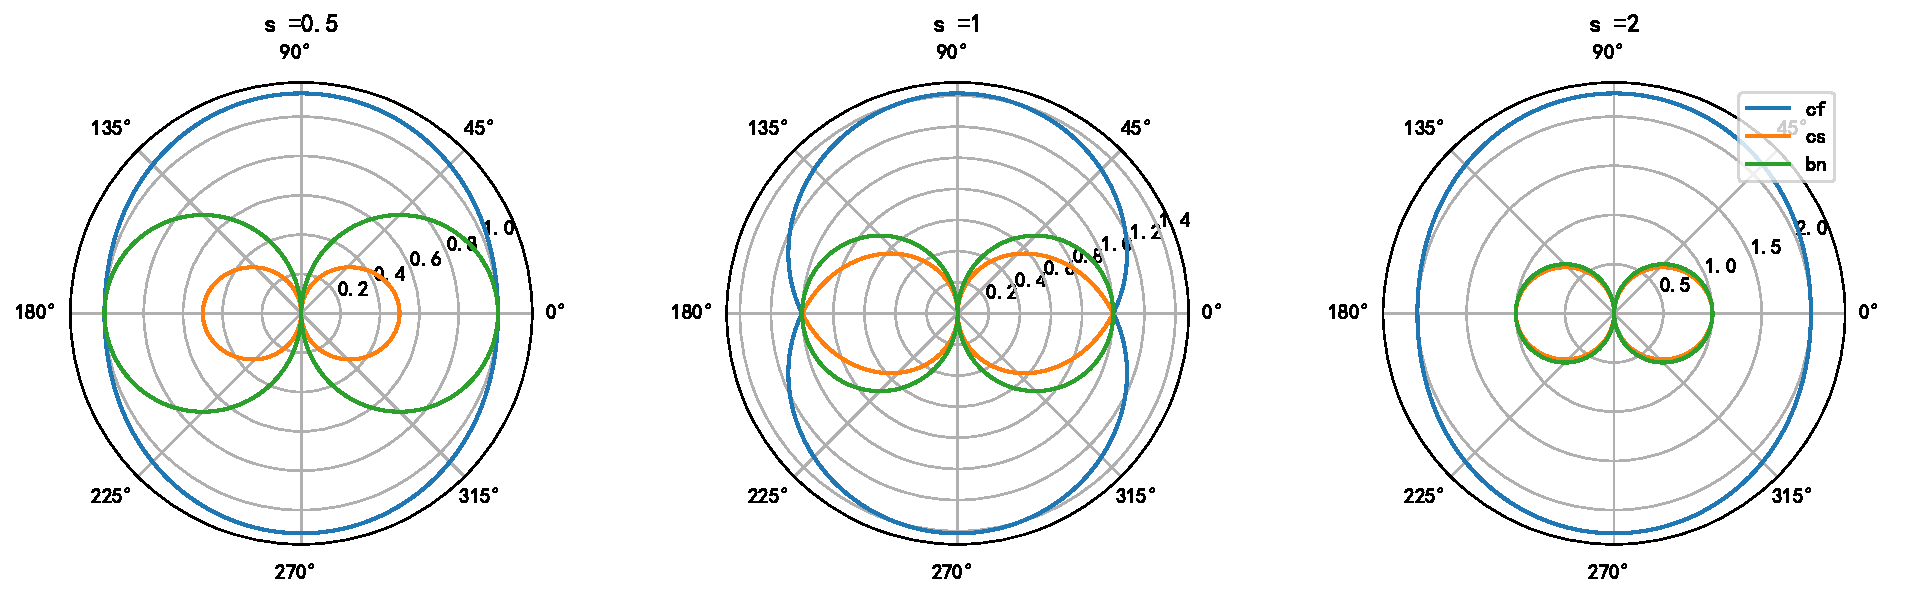
\includegraphics[width=.9\textwidth]{figures/problem1.pdf}
\caption{Illustration of the surface of normal speeds for (a) $s = 0.5$, (b) $s=1$, and
(c) $s=2$.}\label{Friedrich}
 \end{center}
\end{figure}

\subsection{冷等离子体中的色散关系}

磁化冷等离子体的色散关系可以表示为\citep{Diver2001}
\begin{align}
\left(S \sin^2 \theta + P \cos^2 \theta\right) n^4 - \left[R L \sin^2 \theta
+ P S \left(1 + \cos^2 \theta\right) \right] n^2 + P R L= 0 \label{Eqn:Colp}
\end{align}
这里 $n = k c / \omega$ 是折射率, $\theta$ 是波的传播方向和磁场的夹角,
\begin{figure}
%\begin{center}
\begin{tabular}{cc}
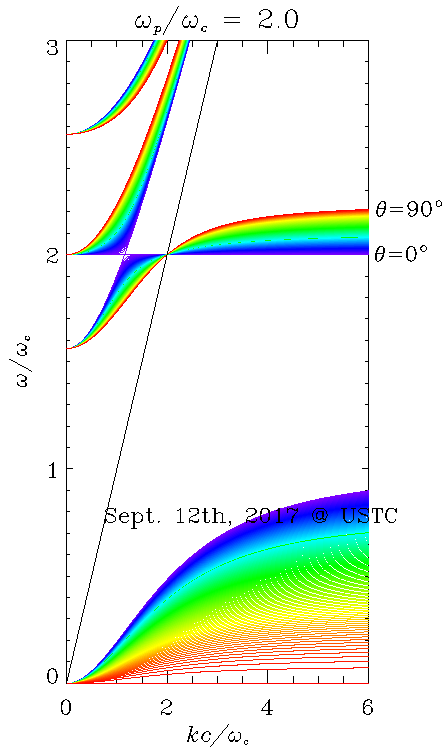
\includegraphics[width=.5\textwidth]{coldp_2_0.pdf} &
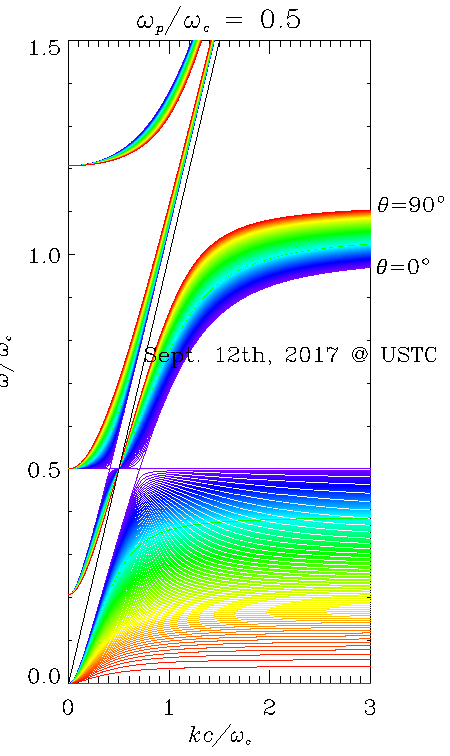
\includegraphics[width=.5\textwidth]{coldp_0_5.pdf}
\\
(a) & (b)
\end{tabular}
\caption{The general dispersion relation for waves in a uniform, magnetised cold
plasma. (a) $\omega_p / \omega_c = 2.0$ and (b) $\omega_p / \omega_c = 0.5$} \label{ColdPlasma}
%\end{center}
\end{figure}
\begin{align*}
S =& (R + L) / 2
\\
D &= (R - L) / 2
\\
R &= 1 - \sum_s \frac{\omega_{ps}^2}{\omega^2} \frac{\omega}{\omega + \omega_{cs}}
\\
L &= 1 - \sum_s \frac{\omega_{ps}^2}{\omega^2} \frac{\omega}{\omega - \omega_{cs}}
\\
P &= 1 - \sum_s \frac{\omega_{ps}^2}{\omega^2}  = 1 - \frac{\omega_p^2}{\omega^2}
\end{align*}
其中 $\omega_{ps}$ 和 $\omega_{cs}$ 分别是第 $s$ 种类粒子的等离子体频率和回旋频率, $\omega_p$ 是整体的等离子体频率. 方程~(\ref{Eqn:Colp}) 还可以写成如下的形式,
\begin{align*}
\tan^2 \theta &= - \frac{P (n^2 - R) (n^2 - L)}{(S n^2 - R L) (n^2 - P)}.
\end{align*}
其中单成分的结果可以参考图~\ref{ColdPlasma}, 进行分析和比较.

\subsection{磁流体力学快磁声激波关系}

磁流体力学快磁声激波关系中\citep{Jeffrey1964}, 用磁场增量 $h_f$ ($h_f \ge 0$)
来表示激波的强度, 通常分析下面的公式
\begin{align}
\frac{X_f^\pm}{h_f} = (B \pm \sqrt{R_X})/C \qquad (\ge 0) \label{Eqn:fShock}
\end{align}
和 $h_f$ 的函数关系. $B$, $C$, 和 $R_X$ 由以下表达式给出,
\begin{align}
B &= (\gamma/2) h_f \sin\theta_0 - (1-s_0),
\\
C &= 2 \sin\theta_0 - (\gamma-1) h_f,
\\
R_X &= B^2 + C(h_f + 2 s_0 \sin\theta_0) \qquad (\ge 0).
\end{align}
其中 $\theta_0$ 为波传播方向和磁场方向的夹角 ($0^\circ \le \theta_0 \le 90^\circ$),
$\gamma=5/3$ 是多方指数. 讨论两种情况, 即 $B$ 在 $C$ 的零点
\begin{align*}
\hat{B} \equiv B(\hat{h}_f) = \frac{\gamma}{\gamma-1} \sin^2\theta_0 - (1-s_0),
\end{align*}
大于等于和小于零的情况, 此处 $\hat{h}_f$ 是 $C=0$ 的根
\begin{align}
\hat{h}_f = \left(\frac{2}{\gamma-1}\right) \sin\theta_0.
\end{align}
具体表现为 $s_0$ 的条件
\begin{align}
s_0 \ge 1 - \gamma \frac{\sin^2\theta_0}{(\gamma-1)},
\end{align}
和
\begin{align}
s_0 < 1 - \gamma \frac{\sin^2\theta_0}{(\gamma-1)}.
\end{align}
而 $\hat{\hat{h}}_f$ 是 $R_X = 0$ 的根,
\begin{align}
& \hat{\hat{h}}_f = \frac{1}{2(\gamma-1) - \frac{1}{2} \gamma^2 \sin^2
\theta_0}\Big\{\sin\theta_0
(2-\gamma)(1+s_0) \nonumber
\\
& \quad + 2\cos\theta_0 \sqrt{(\gamma-1)(1-s_0)^2 + s_0 \gamma^2 \sin^2\theta_0}\Big\}.
\end{align}
将关系~(\ref{Eqn:fShock}) 用图形表示 (可取 $\theta_0$ 的某个典型值进行分析, 如 $\theta_0=15^\circ$),
并参考图~\ref{FShock} 或文献 \citep[第 229 页中的图形]{Jeffrey1964}, 以进行比较.
\begin{figure}
\begin{center}
\includegraphics[width=.9\textwidth]{fShock.pdf}
\caption{Fast shock relation.} \label{FShock}
\end{center}
\end{figure}

\subsection{其他函数}

同学们也可以选其他自己感兴趣或 (专业) 相关的函数进行编程和作图. 说明函数的来源, 可能包含的物理性质, 及其中的一些结果和讨论.

\section{交叉参考}
交叉参考和文献引用也可以参考 \LaTeX 相关文档, 关于公式, 图/表的引用, 直接参考本文文档. 关于文献, 这里有两种做法, 一是用 BibTeX, 文献管理单独用一个文件,
可以注意到, 文献数据库附件文件里的文献还包含了这个作业里面没有引用的文献. \LaTeX 通过 BibTeX 编译时会自动过滤掉, 只将引用的文献列进来. 例如
\begin{quote}
\begin{verbatim}
\bibliographystyle{unsrt}
\bibliography{References}
\end{verbatim}
\end{quote}
这里文献文件是 ``References.bib'', 采用 ``unsrt'' 格式引用和排版. 本报告采用这个办法. 另一种是直接用
\begin{quote}
\begin{verbatim}
\begin{bibliography}
...
\end{bibliography}
\end{verbatim}
\end{quote}
请大家看这个报告源文件中见被注释掉的部分. 本文件的这一部分实际上是通过 BibTeX 生成的 *.bbl (此处为 Assign1.bbl) 后粘贴过来的, 这也是一般期刊最后稿件的要求,
因为提交的文件不需要你们自己的整个文献数据库.

\section{分工说明}

郑惠南提供了最初的报告文本, 程序和图形文件. 高新亮对整个文档, 文件清单进行了检查, 确认.

\section{附件}

\begin{enumerate}
\item
assign1.tex--本报告 \LaTeX 文件
\item
assign1.pdf--本报告 PDF 输出文件
\item
assign1.pro--文中图~\ref{Fig:1} 例子所用的 IDL 计算和图形绘制程序
\item
plot1.pdf--图~\ref{Fig:1} 的 PDF 图形文件, 由 IDL 程序生成的 PS 格式图形文件转换而来
\item
Friedrich.pdf--图~\ref{Friedrich} 的 PDF 图形文件, 由 IDL 生成的数据, 再使用 \LaTeX 的绘图宏包生成
\item
  coldp\_2\_0.pdf--图~\ref{ColdPlasma} 的 PDF 图形文件之一 (a), 由 IDL 程序生成的 PS 格式图形文件做边界调整而成再转换而成. 原图的默认边界是坐标轴 (含坐标其他元素,
  刻度, 标题等等) 围起来的区域. 因为角度的注释跑到边界外面了, 直接插进来这一部分不能全部显示出来. 后面的处理类似. 也可以这样做, 在本文件开始的部分使用了宏包
\begin{verbatim}
\usepackage{epstopdf}
\end{verbatim}
这样包含图形时可以直接使用 EPS 格式文件, 在 \LaTeX --- 实际上是 PDFLaTeX (XeLaTeX) --- 编译后生成的是 PDF 文件, 其中的 EPS 图形通过前面所提的宏包转换, 会有 PDF 格式的中间临时文件. 用这些 PDF 文件替换掉 EPS 文件即可.
\item
  coldp\_0\_5.pdf--图~\ref{ColdPlasma} 的 PDF 图形文件之一 (b), 处理方式同前.
\item
FShock.pdf--图~\ref{FShock} 的 PDF 图形文件, 由 IDL 生成并使用 \LaTeX 加注其中的公式生成, 并调整了边界 (EPS 文件头)
\item
References.bib -- 文献文件
\end{enumerate}

% 以下两行是中文文献国家标准的格式, 如果安装了这两个格式, 建议使用它们
% \bibliographystyle{gbt7714-author-year}
% \bibliographystyle{gbt7714-numerical}
%

%\bibliographystyle{unsrt}
\bibliographystyle{apalike}
\bibliography{References}

%\begin{thebibliography}{1}
%
%\bibitem{Diver2001}
%Declan~A. Diver.
%\newblock {\em A plasma formulary for physics, technology and astrophysics}.
%\newblock Wiley VCH, 1st edition, 2001.
%
%\bibitem{Jeffrey1964}
%A.~Jeffrey and T.~Taniuti.
%\newblock {\em Non-Linear Wave Propagation with Applications to Physics and
%  Magnetohydrodynamics}, volume~9 of {\em Mathematics in Science and
%  Engineering - A Series of Monographs and Textbooks}.
%\newblock Academic Press, New York / London, 1964.

%\end{thebibliography}

\end{document}
